%%% LaTeX Template: Two column article
%%%
%%% Source: http://www.howtotex.com/
%%% Feel free to distribute this template, but please keep to referal to http://www.howtotex.com/ here.
%%% Date: February 2011

%%% Preamble
\documentclass[	DIV=calc,%
							paper=a4,%
							fontsize=11pt,%
							twocolumn]{scrartcl}	 					% KOMA-article class

\usepackage[backend=bibtex]{biblatex}         % Citations
\bibliography{main}

\usepackage[english]{babel}										% English language/hyphenation
\usepackage[protrusion=true,expansion=true]{microtype}				% Better typography
\usepackage[pdftex]{graphicx}									% Enable pdflatex
\usepackage[svgnames]{xcolor}									% Enabling colors by their 'svgnames'
\usepackage[hang, small,labelfont=bf,up,textfont=it,up]{caption}	% Custom captions under/above floats
\usepackage{epstopdf}												% Converts .eps to .pdf
\usepackage{subfig}													% Subfigures
\usepackage{booktabs}												% Nicer tables
\usepackage{fix-cm}													% Custom fontsizes

\usepackage[utf8]{inputenc}                 % Unicode input


%%% Custom sectioning (sectsty package)
\usepackage{sectsty}													% Custom sectioning (see below)
\allsectionsfont{%															% Change font of al section commands
	\usefont{OT1}{phv}{b}{n}%										% bch-b-n: CharterBT-Bold font
	}

\sectionfont{%																% Change font of \section command
	\usefont{OT1}{phv}{b}{n}%										% bch-b-n: CharterBT-Bold font
	}



%%% Headers and footers
\usepackage{fancyhdr}												% Needed to define custom headers/footers
	\pagestyle{fancy}														% Enabling the custom headers/footers
\usepackage{lastpage}

% Header (empty)
\lhead{}
\chead{}
\rhead{}
% Footer (you may change this to your own needs)
\lfoot{\footnotesize Exploratory data analytics for the digital humanities}
\cfoot{}
\rfoot{\footnotesize page \thepage\ of \pageref{LastPage}}	% "Page 1 of 2"
\renewcommand{\headrulewidth}{0.0pt}
\renewcommand{\footrulewidth}{0.4pt}



%%% Creating an initial of the very first character of the content
\usepackage{lettrine}
\newcommand{\initial}[1]{%
     \lettrine[lines=3,lhang=0.3,nindent=0em]{
     				\color{DarkGoldenrod}
     				{\textsf{#1}}}{}}



\bibliography{main}


%%% Title, author and date metadata
\usepackage{titling}															% For custom titles

\newcommand{\HorRule}{\color{DarkGoldenrod}%			% Creating a horizontal rule
									  	\rule{\linewidth}{1pt}%
										}
%%begin novalidate
\pretitle{\vspace{-30pt} \begin{flushleft} \HorRule
				\fontsize{50}{50} \usefont{OT1}{phv}{b}{n} \color{DarkRed} \selectfont
				}
\title{Exploratory data analytics for the Digital Humanities}					% Title of your article goes here
\posttitle{\par\end{flushleft}\vskip 0.5em}

\preauthor{\begin{flushleft}
					\large \lineskip 0.5em \usefont{OT1}{phv}{b}{sl} \color{DarkRed}}
\author{Christopher York, }											% Author name goes here
\postauthor{\footnotesize \usefont{OT1}{phv}{m}{sl} \color{Black}
					Yale University 								% Institution of author
					\par\end{flushleft}\HorRule}
%%end novalidate
\date{}																				% No date



%%% Begin document
\begin{document}
\maketitle
\thispagestyle{fancy} 			% Enabling the custom headers/footers for the first page
% The first character should be within \initial{}
\initial{L}\textbf{orem ipsum dolor sit amet, consectetuer adipiscing elit. Aenean commodo ligula eget dolor. Aenean massa. Cum sociis natoque penatibus et magnis dis parturient montes, nascetur ridiculus mus. Donec quam felis, ultricies nec, pellentesque eu, pretium quis, sem.}

\subsection*{The Comédie Française Registers Project}
Boilerplate info on the CF and the CFRP: who, what, why, how.

Lorem ipsum dolor sit amet, consectetuer adipiscing elit. Aenean commodo ligula eget dolor. Aenean massa. Cum sociis natoque penatibus et magnis dis parturient montes, nascetur ridiculus mus. Donec quam felis, ultricies nec, pellentesque eu, pretium quis, sem. Nulla consequat massa quis enim. Donec pede justo, fringilla vel, aliquet nec, vulputate eget, arcu. In enim justo, rhoncus ut, imperdiet a, venenatis vitae, justo. Nullam dictum felis eu pede mollis pretium. Integer tincidunt. Cras dapibus. Vivamus elementum semper nisi. Aenean vulputate eleifend tellus. Aenean leo ligula, porttitor eu, consequat vitae, eleifend ac, enim. Aliquam lorem ante, dapibus in, viverra quis, feugiat a, tellus. Phasellus viverra nulla ut metus varius laoreet. Quisque rutrum. Aenean imperdiet. Etiam ultricies nisi vel augue. Curabitur ullamcorper ultricies

\subsection*{Exploratory Data Analysis and Data Visualization}

Imagine a student, perhaps in an undergraduate class on theater history, who uses the tool to explore the Comédie-Francaise Registers dataset while writing a paper. The student may have some background knowledge from an introductory lecture.  She knows that Louis XIV issued a royal decree founding the Comédie-Française in August 1680, that together with the Comédie Italienne and the Opéra the troupe occupied a central place in French stage tradition, closely associated with the foundational figures of Molière and Racine, and notable for its close association with the French court.  She may have privately noted a contrast between English Restoration theater’s fragmentation and the Comédie-Française’s remarkable institutional persistence and continuity, offering performances every season from founding, throughout the upheaval of the French Revolution and into the 21st century.

However, beyond this rough outline the overall shape of the Comédie-Française Registers dataset will be completely unclear to a newcomer like our hypothetical student.  Which were the prominent authors and plays? Were ticket sales consistent across the years?  Did plays stay in the repertory, or did it change every year?  What dates did the theater season run?  Which plays were typically performed together in an evening?

\begin{figure}
  \centering
  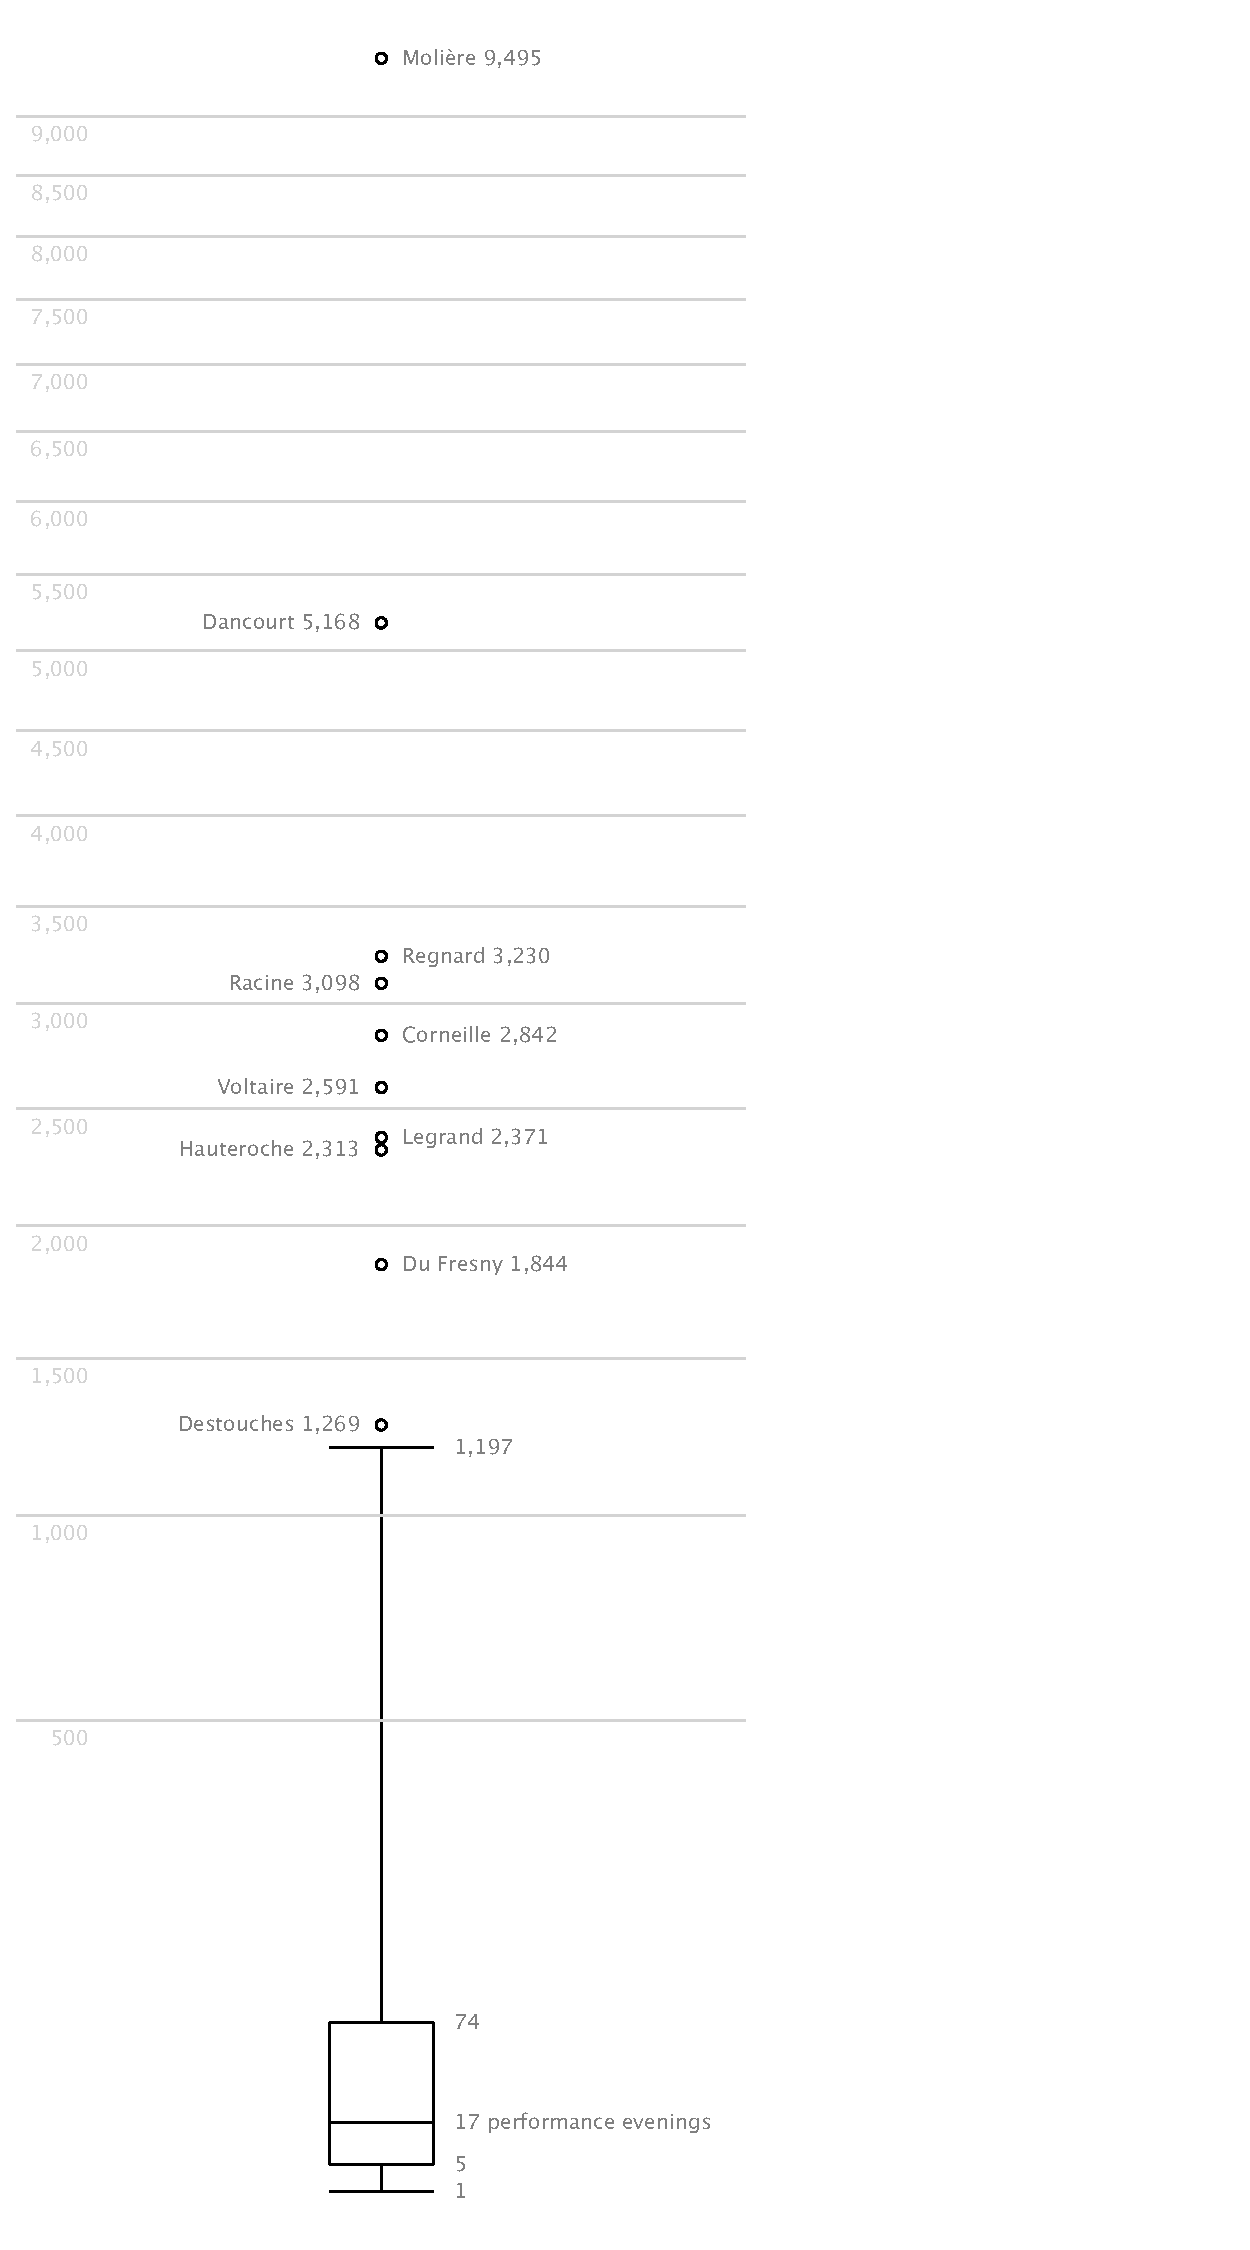
\includegraphics[height=9in]{viz/author_performances.pdf}
	\caption{Major authors by number of evenings performed}
  \label{fig:tukey_boxplot}
\end{figure}

Giving a sense of the overall landscape, while also providing opportunities to drill down and inspect specific features is a task in exploratory data analysis. This term, introduced by John Tukey in his 1977 book of the same title, encompasses a collection of techniques for identifying the main characteristics of a novel dataset, about which one may initially know nothing.  Tukey contrasted this exploratory process of surveying the data landscape and forming some initial hypotheses to confirmatory data analysis, the subsequent task of using data to confirm or disprove a hypothesis one has already formulated.\cite{TUKEY:1977}  The CFRP analytics site (http://christopheryork.github.io/cfrp-analytics/; http://cfregisters.org/app), which our theater student might use to generate many of the examples in this paper, was conceived as a general-purpose tool to enable users without a background in statistics to do basic exploratory data analysis—to formulate hypotheses, do confirmatory data analysis to test them, and then primary source critique to confirm that hypotheses are well-supported by the Comédie-Française’s archival resources.  It is this balance between data analysis and source critique that makes the CFRP analytics tool unusual, bridging statistics and the humanities.

Before we delve into description of the CFRP analytics tool, let’s pause first to consider potential visual displays for exploratory data analysis, so as to have a sense of the design space. Suppose our student has decided her best way into the Comédie-Française Registers data is to look at authors.  What sort of visualization can answer these questions: Which were the most prominent and influential?  How did minor authors fare in the repertoire?  What were the major periods, and how often did authors remain popular across periods?

When Tukey proposed exploratory data analysis as a field, he envisioned using visuals based on descriptive statistics as the primary entry point to new datasets.  For example, our student could start with the Tukey boxplot below, which uses the number of evenings the Comédie Française performed a play by the given author as a rough proxy for authorial importance.  Despite its visual spareness, the graph is information-rich, sketching the outlines of an theater troupe that experimented restlessly with new authors’ work but viciously dispatched unsuccessful ones after a few nights of poor performance; all the while staging works by the most successful authors over and over again. Of the 314 non-anonymous authors or co-author teams whose work played at the Comédie-Française between 1680-1793, fully 25\% had work in-theater for only 1 to 5 evenings (lower box edge).  Half of all authors saw 17 or fewer performances (median, the box’s center line), and 75\% of authors’ work had less than a full season’s time on the stage.  Clearly, success at the Comédie-Française was a vanishingly rare phenomenon.

At the upper end of the scale, Tukey’s visualisation singles out some outlier authors whose work was spectacularly successful.  Our student, while perhaps prepared for Molière’s pre-eminence, might be struck by the degree to which he dominated the Comédie-Française’s daily repertoire (note the exponential scale: Molière was performed fully twice as many nights as next-in-line comedian of manners Florent Carton Dancourt).

The striking success of Tukey’s visualisation lies in its balance between conveying the lay of the land—a large body of unsuccessful authors—while also singling out notable landmarks: individual authors whose work did succeed, and famously.  From this bit of exploratory data analysis, our imaginary student could begin formulating an overarching narrative while also following up on novel outlier authors whose names are unknown but whose success was clear: Destouches, Du Fresny, Hauteroche, Legrand, and so on.

Against the boxplot’s virtues, one can balance a number of demerits.  It is visually unsatisfying, rich in statistical implications but poor in visual detail that encourages users to look up new facts in a known resource.  Its very flexibility—we could be researching the distribution of genres, the profitability of individual plays, or variations in ticket price—begs for a visualisation tailored to the Comédie-Française alone.

Let us follow our hypothetical student to explore the top-performed Comédie-Française authors using a purpose-built visualisation for analysing repertoire (see figure 2).  For each play by the 10 authors whose work was performed by the Comédie-Française more than 1,200 nights, this graph marks the number of performances per year onward from the premiere in a vertical line.  Stark differences in authorial profile and professional trajectory appear, which the previous graph had glossed over.  It becomes clear how dependent the Comédie-Française was on a canon of work already established before the formation of the troupe.  Of the authors whose plays were revived consistently, year on year through the troupe’s history, the lion’s share appear in the pivotal 1680-81 season: a large body of work by Molière, Pierre Corneille and Racine (at left).  Only Jean-François Regnard, gambler, adventurer and former slave turned playwright, was able to consistently introduce new hit plays that were revived year-on-year.  Voltaire, it becomes clear by comparison, only hit his stride in mid-career with Zaïre in 1732; his later plays languished, premiered but un-revived.

From a purpose-built visualisation such as this, our hypothetical student might make any number of observations that open doors into individual authors’ professional careers.  Pierre Corneille’s frustrated later-life failures are clearly visible; as is Dancourt’s unique authorial signature as a fount of works consistently premiered year on year, yet only intermittently canonised.  Likewise, Abraham-Alexis Quinault’s (also known as Dufresne) status as the one-hit wonder author of Esprit de Contradiction is confirmed.  More subtly, one sees the gradual shift in taste away from classical models, from Molière’s singular dominance of repertory through 1720, to a more tepid (but consistent) series of revivals after 1750—just as Voltaire’s work achieved dominance.

The heatmap’s visual richness and usefulness for investigating authorial history hide faults that make it quite unsuitable for exploratory data analysis.  As noted above, a cardinal virtue of the author performance boxplot was balance between giving a sense of the ``landscape'' of all authors’ performance histories while simultaneously singling out notable features: ten particularly well-performed authors.  The heatmap’s balance of dark and light suggests similar reading—but deceptively.  Because it does not include all plays performed through the 113-year sequence of the Comédie-Française dataset, it gives little sense of why these are of particular interest: where, how many, and what characterised the unsuccessful authors.  It is a picture of some tall trees in isolation from the surrounding forest.  One might think that including every play and ordering them in sequence chronologically by premiere would counteract this (see figure below for an excerpt from 17xx-17yy).  While it does accurately suggest the balance between often-performed plays dating from the years of the troupe’s founding and rarely-revived plays that premiered later, to see this effect we must order by the year each play’s premiere and so lose the grouping by author.  Some of the most important features of the dataset disappear: for example, Voltaire’s dominance of the post-1730 repertoire is completely hidden, since his successful plays are scattered among many less-successful ones by other authors.

Perhaps more damning, a repertoire heatmap above is a special purpose visualisation, crafted to expose a fixed set of patterns but difficult to adapt to other categories of analysis.  Changing it to look at the genre of plays performed over time, or variations of what is played during a week, would basically require starting over with a novel programming task.  By contrast, during the process of exploratory data analysis, users are likely to want to experiment with many different aggregations and graphs in a short period of time—for example, to see ``were plays of a different genre performed in later decades?'' or ``were different weekdays associated with different genres?''  Despite involving the same variables—time and genre of play performed—these two questions lend themselves to different analyses and graphs.  This is because ``decade of performance'' is a linear and continuous aspect of the data, while ``weekday of performance'' is cyclical and discrete.

\subsection*{Goal and Design Constraints: General vs Special-Purpose Tools}

A digital humanist with specialist skills in statistics and data visualisation, given the Comédie-Française dataset and a research question like the ones above, might produce any number of compelling purpose-built visuals that speak compellingly to questions like ``how did genre vary by weekday'' or ``which were prominent authors performed by the troupe?''  The challenge for an exploratory data analysis tool, however, is to enable the non-specialist user to probe any number of different questions using general-purpose visuals.  (For one potential starting list of questions for the Comédie-Française dataset, see the sidebar).

Doing so involves comparing any number of different aspects of the dataset in quick succession, digging for suggestive features and large-scale patterns, formulating, testing and rejecting many hypotheses.

The tool works by progressive refinement of the dataset, to expose distributions of the data points across a number of dimensions (listed in the sidebar, right).  Let us follow the prior query through, to show how our student user might use the tool to explore the problem of determining the main authors in the Comédie-Française’s repertoire, their periods and relative importance.  To begin, our student would select an aggregate value of interest: for example, the number of performances; gross receipts; average price of tickets sold; or average receipts per night.

As seen in the Tukey boxplot we considered first, number of performances is a good initial metric indicating the prominence of an author in the repertoire.  On choosing this, our student sees the entire dataset aggregated by number of nights performed: over the 114-year period covered by the dataset, the Comédie-Française performed 34,904 nights (step 1, right).  At about 306 live evenings per year (34,904 / 114), this already gives some indication of the theater’s preternatural activity.  Was the Comédie Française pressed to maintain profitability by keeping its doors open and attendance consistently high, a stress familiar to 20th century theater owners?  Our student investigator does not know; but already a field of questions is opening up that supplements her initial interest in repertoire.  What role did prominent authors play in maintaining the Comédie Française’s yearly schedule?

Our student decides to take a quick look at how the number of performances varied over the course of the theater’s history.  From the list of available dimensions, she elects to divide the existing result by decades (step 2).  This will give a sense of how performances were distributed through history (step 3).  While this is an obvious—and good—choice, our student could have chosen to drill down into the dataset using any of the other dimensions available: to see which genres were performed more nights, for example, or to find the most (or least) popular play titles by number of performances.

Seeing results in tabular form can be useful, particularly when one delves deep into a particular problem or research question.  A visual presentation gives more immediate meaning to the same set of numbers, however.  From here, we will follow the student as she does exploratory data visualisation using the tool’s graph component, which she accesses by choosing the leftmost results panel (step 4).

The graph of number of performances by decade is immediately more suggestive than the table of numbers.  The much lower number of performances in the 1790s immediately stands out, but even more striking is the slight fall in activity at 1720, which is only gradually rises back to its original levels at the turn of the 19th century.  However, our student is immediately struck by the years immediately preceding the French Revolution, when it is clear the theater thrived.  Is it possible, the Comédie Française was involved in and benefited materially from the intellectual and political turmoil of the Enlightenment?

Perhaps this question will become clearer as our student pursues her original interest in the Comédie Française’s prominent authors.  She chooses to divide the current query on performance evenings per decade further, this time by the authors of the plays performed.

She chooses the default option for ``author'' (authorn, explained further below) in the table’s columns.  This generates a table of number of performances for each author, divided by decade.  Because there are 314 columns in this table, it is excerpted in the figure for step 5 (following page).

Subtotals tallied by author appear at the lower margin of the table, and tallied by decade at the right margin; the lower right cell tallies performances for the entire table.  Authors are ordered alphabetically across the top, such that as the user scrolls horizontally, it is possible to detect from visual density of the figures which were the prominent authors, and in which decades.  In this table, for example, Voltaire’s dominance of the repertoire from the 1730s onward is immediately obvious.

Visual inspection only conveys a rough sense of the historical distribution of performances between authors, however.  It would be more helpful to know immediately which were the most- and least-performed authors.  To accomplish this, the student sorts the table by column (author name), as seen in step 6.  Here, we begin to see the outlines of the vital descriptive statistics that John Tukey foregrounded in his boxplot.  As can be seen by comparison with figure \ref{fig:tukey_boxplot}, the sorted crosstab table identifies notable outlier datapoints along a dimension.  From here, our student can begin making interpretive inferences like those we pointed out in our discussion of Tukey’s boxplot: Molière’s central place in the repertoire is immediately obvious, as is the prominence of the other foundational authors like Racine and Corneille right from 1680.  Moreover, some of the phenomena we observed in the custom-tailored heatmap (figure 2) are evident here, but hidden in the boxplot: for example, Voltaire’s gradual rise to fame at 1750, when his importance in the repertoire superceded that of Racine and Corneille together.  (By sorting the table in the opposite order, low-to-high by columns, our student can also explore the least-performed authors, exposing  the fragmentation and churn we noted in the Comédie Française repertoire using Tukey’s boxplot.)

One of the cardinal advantages of the Tukey boxplot, as we noted, lay in giving a sense both of absolute numbers of performances for each author, as well as how those numbers compared with the body of other authors in the repertoire.  While the table format, with fixed ordinal positions for rows and columns, cannot mimic this graphically, it can convey a sense of the importance of each value within the population of an entire row or column.  Doing this enables our student to compare the relative prominence of high-performed authors to each other, and to the entire population of authors per decade (step 7).  Here she sees her intuitions about the troupe’s dependence on Molière confirmed: fully 28% of all nights through the run saw the performance of a Molière play (lower-right corner), as against 7.6% of all nights for Voltaire.  More importantly, she now has a sense of the significance of Voltaire’s rise after 1750: in this and succeeding decades, between 14-16% percent of all nights involved a performance of one of his plays.  However, decade by decade through Voltaire’s heyday, it becomes clear that Molière plays still formed a higher proportion of the repertoire.  Looking at the top-performed authors as a group makes this conservative phenomenon even further.  The top 6 authors appeared on fully 60-80% of all nights!  [ double check that this works with author_n ]

Looking back at our student’s progress using cross-tabulations, it is clear her insights are built on three vital features.  First, the ability to divide the dataset by more than one dimension (in this case, by author and time rather than just author).  Second, sorting from high-to-low and low-to-high values on an axis make it easy to locate the top and bottom performers (these are generally Tukey’s statistically-significant outliers).  This enabled our student to identify notable authors without having to scan the entire table. Third, showing computed aggregates ranked as proportion of a row or column of the data gives a sense of how important each value is vis-a-vis its neighbors.  Hence our student could judge the relative prominence not only of Voltaire to Molière, but also each of these authors compared with the unseen collection of all Comédie-Française authors.

Shortcomings of the table format quickly appear, however, if our student moves from comparing authors performances by decade to each other, to comparing authors’ performances rates in one decade to those in others.  When, for example, was the peak in Comédie-Française performances and did it correlate with a particular author?  To begin looking at this question, the student changes the table above to order and calculate percentages within columns rather than rows (step 8).

While the display conveys the information our student seeks—which decades saw the most open performances, broken down by author—it feels incoherent, because unlike ``author’s name'', ``time'' has a natural order and we expect to always see data presented in that order, even when seeking minima and maxima.

Discuss line graphs of tables, ordering and selection of top 10 items

Discuss future improvements:  include quantile points


[ Exposing important features of the statistical landscape: top-n peaks versus Tukey’s boxplot (figures 1 \& 2)

\subsection*{Drill-down: calendar}

In an article from 1996, ``The Eyes Have It'', Ben Schneiderman introduced his influential visual information seeking mantra: ``Overview first, zoom and filter, then details on demand.''\cite{Shneiderman:1996}  The mantra identifies one successful narrative dynamic for information discovery in large datasets, in which the user first views an overview of the data ``landscape'', then pursues phenomena of particular interest by zooming in on a regional sample or filtering the entire dataset using search criteria.  At this point the user is likely to want to confirm individual data points by clicking to bring up ``details on demand.''  From here, the process loops back iteratively as necessary to examine other slices of the data landscape that support or disprove the insight being exploring, but using other data points.

Certainly Scheiderman’s mantra applies to general-purpose use of CFRP’s Crosstab table, as users select data categories, filter or scroll down to particular columns or rows of interest, and mouse over individual table cells to see details of a particular aggregate.  However, the CFRP Crosstab tool was designed to support Schneiderman’s information seeking mantra in a fashion shaped by the particular concerns of humanities research.

The CFRP Crosstab’s calendar function leverages characteristic feature of the Comédie Française registers: with only one performance session per day, the Comédie Française dataset can be arranged to expose the one-to-one correspondence between dates and archival pages.  So, on switching from the table view to the calendar (see figure above), one sees the same data aggregation, but mapped in quantiles by day.  From here one can zoom in on a specific range of days by highlighting them.

[ patterns of performance by weekday: genre and comedy / tragedy

Simultaneously, the calendar enables users to take one step away from aggregate values towards the physical sources, by breaking each cell in the crosstab table into days.  For example, (see figure below…)

[ drill-down on individual cells in the table of crosstab results: 1680s Pierre Corneille receipts

More importantly, however, from here the ``details on demand'' pull up individual archival pages for the performance session on a given day.  This allows the user to confirm computer analyses by direct inspection of archival sources...

\subsection*{Primary Resource Confirmation: the Register Image Viewer}

References to Martha Howell \& Walter Prevenier, From Reliable Sources...

\section*{Heading on level 1 again}
Lorem ipsum dolor sit amet, consectetuer adipiscing elit.

\subsection*{Problems and Perspectives}

\begin{description}
	\item[First] missing funds, from Greg Brown’s publications; missing information on seating categories: demographic, class inferences difficult
	\item[Last] This is the last item
\end{description}

\begin{itemize}
	\item First item in a list
	\item Second item in a list
	\item Third item in a list
\end{itemize}

DH datasets never complete

DH datasets demand foreign expertise
  [ real vs historical values: from economic history

DH datasets mismatch established business models for data
  [ analysis of receipts data: line-item information on modern receipts versus multiple bills (in CF and studio-system Hollywood)

...

\printbibliography

\end{document}
